\section{Theory}
\label{sec:theorie}

To reasonably discuss the experiment's execution as well as later evaluate the measurements, some theoretical basics are needed.

\subsection{X-rays}

The term X-ray describes electromagnetic radiation with an energy of around $\SI{1}{\kilo\eV}$ to $\SI{100}{\kilo\eV}$ \cite{gamma}.
As shown in \autoref{fig:xraytube}, one possibility of producing such radiation is through the use of an X-ray tube.

\begin{figure}[H]
    \centering
    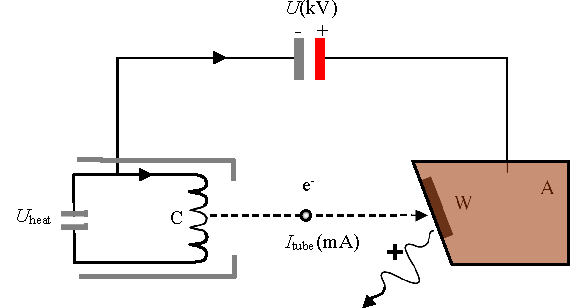
\includegraphics{figures/x-ray_tube.pdf}
    \caption{Schematic view of an X-ray tube with cathode C and anode A \cite{xraytube}.}
    \label{fig:xraytube}
\end{figure}

A wire is heated by a voltage $U_\text{heat}$ until it becomes incandescent.
Thus, it emits electrons, which are then accelerated towards the anode through a high voltage between cathode C and anode A.
When they hit the anode material, they lose energy through interaction, namely through bremsstrahlung and ionisation.
While bremsstrahlung is emitted as a continuous spectrum, the X-rays created by ionisation posses a characteristic and discrete wavelength. \\

X-rays behave differently when passing through and being reflected by different materials.

\subsection{Single-interface Refraction}

When hitting a single flat surface, the refractive index for X-rays can be described by
\begin{equation}
    n = 1 - \delta + i\beta \,.
    \label{eq:refractiveindex}
\end{equation}
The terms $\delta$ and $\beta$ describe a dispersion an absorption term with $\delta > 0$ and $\beta \propto \mu$ where $\mu$ is the linear
absorption coefficient. \\
The process of Refraction and reflection is shown in \autoref{fig:singleinterface}.

\begin{figure}[H]
    \centering
    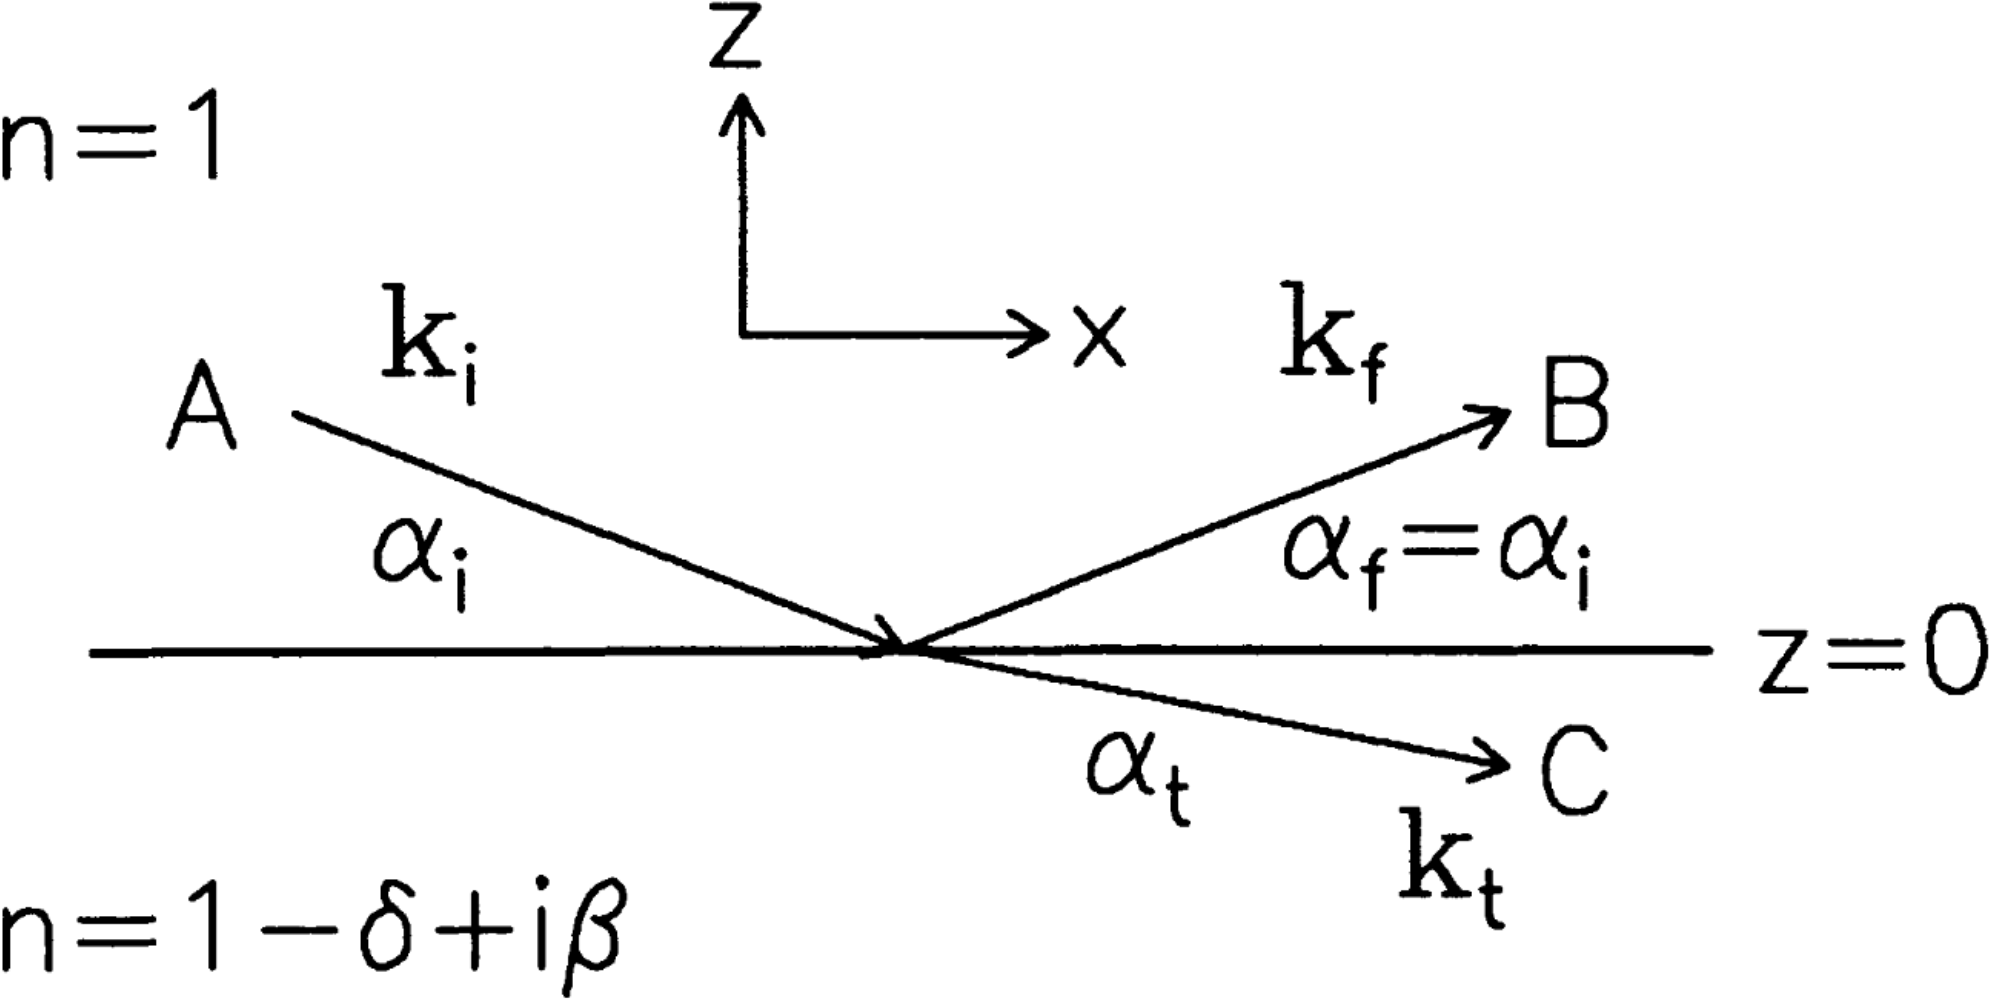
\includegraphics[width=.9\textwidth]{figures/scattering.png}
    \caption{Refraction and reflection of a plane electromagnetic wave on a flat surface with grazing angle $\alpha_\text{i}$, 
    reflection angle $\alpha_\text{f} = \alpha_\text{i}$ and transmission angle $\alpha_\text{t}$ \cite{tolan}.}
    \label{fig:singleinterface}
\end{figure}

With $\delta \sim 10^{-6}$ and $\beta \sim 10^{-7}$ it can be seen that $|n| < 1$, although it may still be close to $1$.
This means that, for angles below a critical angle $\alpha_\text{c}$, total reflection is possible.
Assuming the exit angle $\alpha_\text{t}$ of the refracted beam to be zero, the critical angle is given by
\begin{equation}
    \alpha_\text{c} \approx \sqrt{2\delta} = \lambda \sqrt{\frac{r_\text{e} \rho}{\pi}} \,,
    \label{eq:critangle}
\end{equation} 
where $r_\text{e}$ is the classical electron radius, $\rho$ the electron density and $\lambda$ the wavelength of the X-ray photon \cite{tolan}. \\

In order to now describe the amplitude of transmitted and reflected X-rays, we use the Fresnel equations.
Normally, for different polarisations of photons, different equations apply.
But here, since the refractive indices $n_1$ and $n_2$ of the vacuum and medium are almost identical (with corrections at $\mathcal{O}(10^{-6})$),
the different equations are identical. \\
For the reflected amplitude,
\begin{equation}
    r = \frac{n_1 \cos \alpha_1 - n_2 \cos\alpha_2}{n_1 \cos \alpha_1 + n_2 \cos\alpha_2}
    \label{eq:reflectedamplitude}
\end{equation}
holds while the transmitted amplitude is described by
\begin{equation}
    t = \frac{2 n_1}{n_1 \cos \alpha_1 + n_2 \cos\alpha_2} \,.
    \label{eq:transmittedamplitude}
\end{equation}
The angles $\alpha_1$ and $\alpha_2$ describe the angles of the reflected and namely transmitted light. \\

These formulae allow us to calculate the so-called Fresnel reflectivity $R_\text{F} = |r|^2$, which becomes
\begin{equation}
    R_\text{F} \simeq \left(\frac{\alpha_\text{c}}{2\alpha_i}\right)^4
    \label{eq:fresnelreflectivity}
\end{equation}
for incident angles $\alpha_i > 3 \alpha_\text{c}$ \cite{tolan}.


\subsection{Multi-interface Refraction}

Until now, we have only looked at refraction of X-rays on a single interface surface.
If the X-ray, or any electromagnetic radiation, instead hits a layered system, as seen in \autoref{fig:multilayeredsystem}, the radiation is refracted and transmitted at every single layer.

\begin{figure}[H]
    \centering
    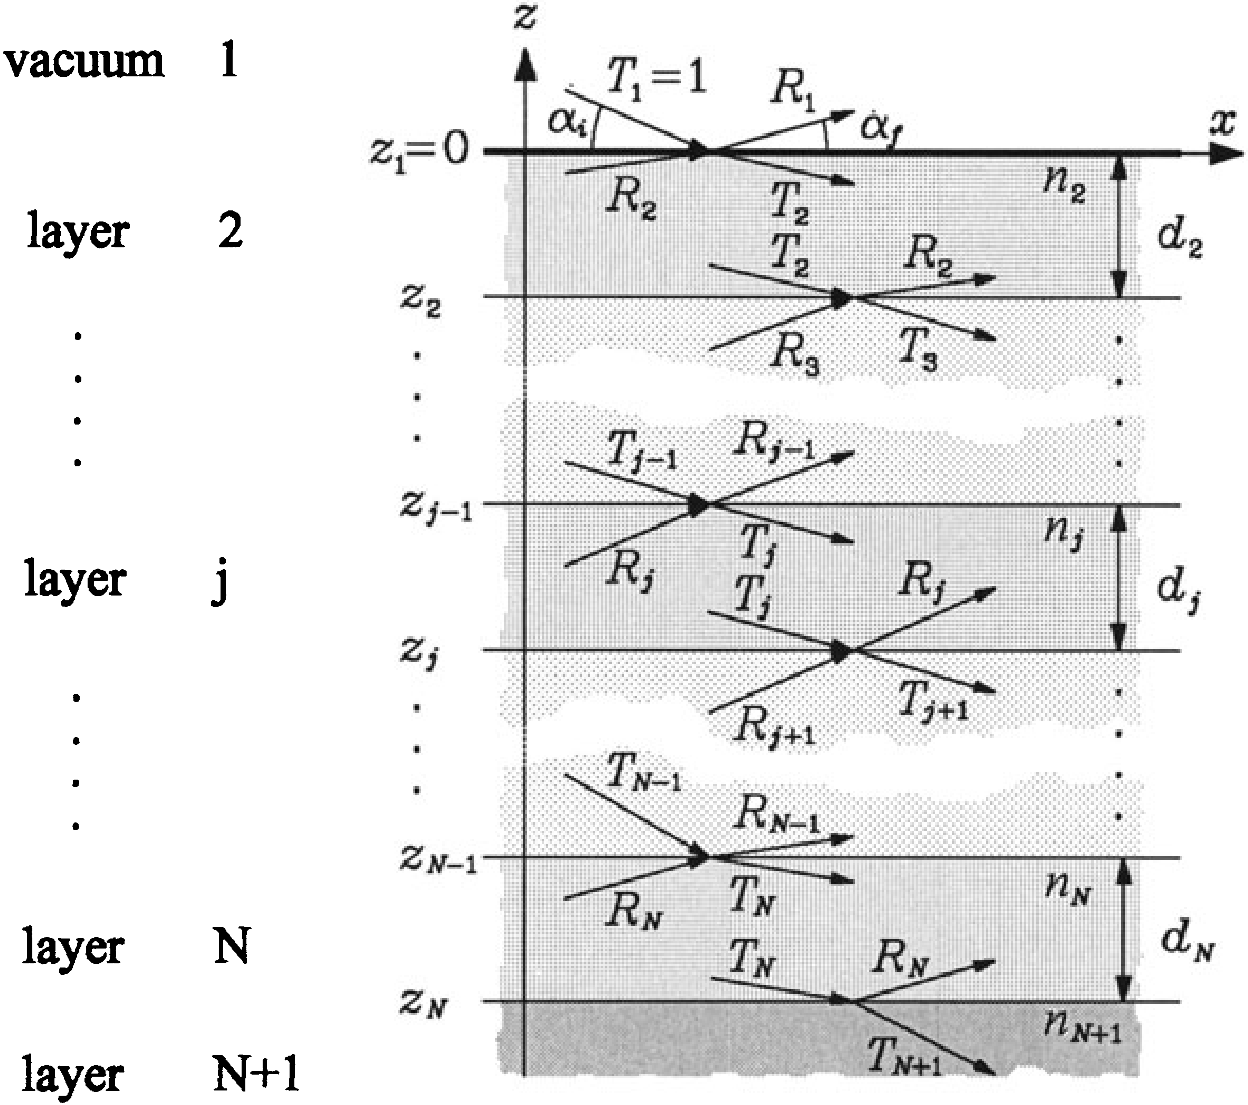
\includegraphics[width=.5\textwidth]{figures/multi_layer.png}
    \caption{Refraction and reflection of a plane electromagnetic wave inside a $N+1$-layered system \cite{tolan}.}
    \label{fig:multilayeredsystem}
\end{figure}
This also means that the transmitted rays from one layer can interfere with the reflected radiation from a deeper layer, 
causing oscillations in the systems reflectivity.
These so-called \textit{Kiessig oscillations} are shown in \autoref{fig:kiessigoscillations} and in turn can be used to calculate the layer thickness.
With the z-component of the wave vector transfer $q = \vec{k}_\text{f} - \vec{k}_\text{i}$, $q_\text{z} = 2 k \sin\alpha_i$, the layer thickness is
\begin{equation}
    d = \frac{2\pi}{\Delta q_\text{z}} \approx \frac{\lambda}{2 \Delta \alpha_i} \,.
    \label{eq:layerthickness}
\end{equation} 

\begin{figure}[H]
    \centering
    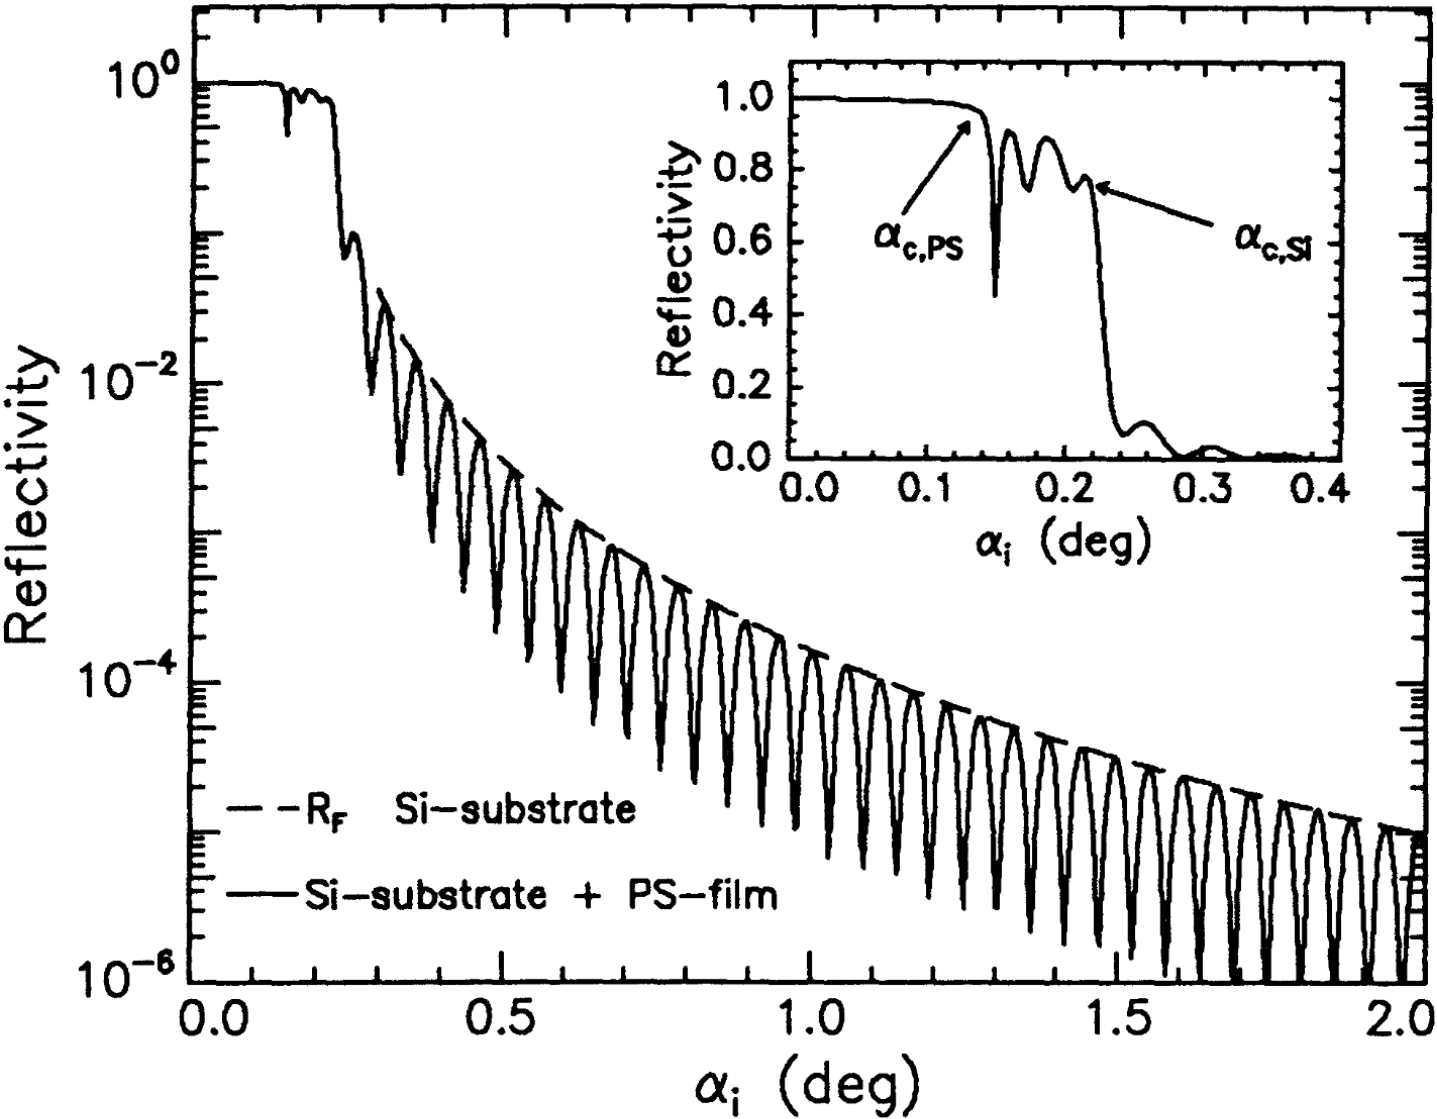
\includegraphics[width=.5\textwidth]{figures/kiessig_oszillation.png}
    \caption{Graphic representation of Kiessig oscillations inside a multi-layered system with critical angles shown for polystyrene (PS) film and Si \cite{tolan}.}
    \label{fig:kiessigoscillations}
\end{figure}

To calculate the Kiessig oscillations, the lowest layer is taken as a layer with infinite thickness without reflection from below, meaning $R_{N+1} = X_{N+1} = 0$.
The rest of the layers is then recursively calculated from the bottom up, giving the recursive formula
\begin{equation}
    X_j = \frac{R_j}{T_j} = \exp(-2i k_{z,j} z_j)\frac{r_{j,j+1} + X_{j+1} \exp(2i k_{z,j+1} z_j)}{1 + r_{j,j+1} X_{j+1} \exp(2i k_{z,j+1} z_j)} \,,
    \label{eq:parrattalgo}
\end{equation}
where
\begin{equation*}
    r_{j,j+1} = \frac{k_{z,j} - k_{z,j+1}}{k_{z,j} + k_{z,j+1}}
\end{equation*}
is the Fresnel coefficient of the $j$-th interface \cite{tolan}.
This approach is called \textit{Parratt algorithm}.

\subsection{Rough Surfaces}

Real surfaces are seldom even.
So we take an ensemble of even surfaces to approximate the rough surface as seen in \autoref{fig:approxrough} and modify the Fresnel coefficient so that
\begin{equation}
    \tilde{r}_{j,j+1} = r_{j,j+1} \exp(-2 k_{z,j} k_{z,j+1}\sigma_j^2) \,,
    \label{eq:modifiedfresnelfcoefficient}
\end{equation}
where 
\begin{equation*}
    \sigma^2 = \int(z-\mu_j) P_j(z) \text{d}z = \int(z-z_j) P_j(z) \text{d}z
\end{equation*} 
is the root-mean-square roughness for a probability distribution $P_j$, here a Gaussian with mean $\mu_j = z_j$.

\begin{figure}
    \centering
    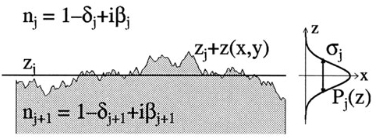
\includegraphics[width=.5\textwidth]{figures/parrott_rough.png}
    \caption{Schematic representation of a rough surface approximated by even surfaces at height $z + z_j$ with probability distribution $P_j$ \cite{tolan}.}
    \label{fig:approxrough}
\end{figure}

It should be noted that this modification works only for systems where the roughness $\sigma_j$ is much smaller than the layer thickness $d_j$.
For systems with greater roughness, the smaller even surfaces must be treated as different layers with their own refractive indices etc. \cite{tolan}.

\subsection{Geometry Factor}

It must also be noted that the beam used in this experiment still has a width $b_\text{i}$.
Especially for small angles, it will cover more are than the sample with length $l$ (shown in \autoref{fig:geometryfactor}), 
which has to be corrected by
\begin{equation}
    G = \begin{cases}
        \frac{D \sin\alpha_\text{i}}{d_0}&, \quad \alpha_ \text{i} < \alpha_\text{g} \\
        1&,\quad \alpha_\text{i} > \alpha_\text{g}
    \end{cases}
    \label{eq:GeometryFactor}
\end{equation}
with total beam width $d_0$ and effective beam area $D \sin\alpha_\text{i}$ \cite{v44}.

\begin{figure}[H]
    \centering
    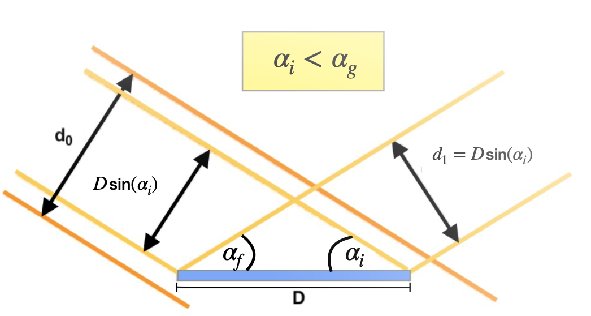
\includegraphics{figures/beam_width.pdf}
    \caption{Schematic view at the beam hitting the sample at a low angle $\alpha_\text{i}$ where the beam area is larger than that of the sample \cite{v44}.}
    \label{fig:geometryfactor}
\end{figure}




